\documentclass[a4paper, 12pt]{article}

%%% Работа с русским языком
\usepackage{cmap}					% поиск в PDF
\usepackage{mathtext} 				% русские буквы в формулах
\usepackage[T2A]{fontenc}			% кодировка
\usepackage[utf8]{inputenc}			% кодировка исходного текста
\usepackage[russian]{babel}	% локализация и переносы

%%% Дополнительная работа с математикой
\usepackage{amsmath,amsfonts,amssymb,amsthm,mathtools} % AMS
\usepackage{icomma} % "Умная" запятая: $0,2$ --- число, $0, 2$ --- перечисление

%% Номера формул
%\mathtoolsset{showonlyrefs=true} % Показывать номера только у тех формул, на которые есть \eqref{} в тексте.

%% Шрифты
\usepackage{euscript}	 % Шрифт Евклид
\usepackage{mathrsfs} % Красивый матшрифт

%% Поля
\usepackage[left=2cm,right=2cm,top=2cm,bottom=2cm,bindingoffset=0cm]{geometry}

%% Русские списки
\usepackage{enumitem}
\makeatletter
\AddEnumerateCounter{\asbuk}{\russian@alph}{щ}
\makeatother

%%% Работа с таблицами
\usepackage{array,tabularx,tabulary,booktabs} % Дополнительная работа с таблицами
\usepackage{longtable}  % Длинные таблицы
\usepackage{multirow} % Слияние строк в таблице

%% Красная строка
\setlength{\parindent}{2em}

%% Интервалы
\linespread{1}
\usepackage{multirow}

%% TikZ
\usepackage{tikz}
\usetikzlibrary{graphs,graphs.standard}

%% Верхний колонтитул
\usepackage{fancyhdr}
\pagestyle{fancy}

%% Перенос знаков в формулах (по Львовскому)
\newcommand*{\hm}[1]{#1\nobreak\discretionary{}
	{\hbox{$\mathsurround=0pt #1$}}{}}

%% Мои дополнения
\usepackage{float} %Добавляет возможность работы с командой [H] которая улучшает расположение на странице
\usepackage{gensymb} %Красивые градусы
\usepackage{graphicx}               % Импорт изображений
\usepackage{caption} % Пакет для подписей к рисункам, в частности, для работы caption*

\begin{document}
	\begin{titlepage}
		\begin{center}
			\large\textbf{Московский Физико-Технический Институт}\\
			\large\textbf{(государственный университет)}
			\vfill
			\huge\textbf{Отчёт о выполнении лабораторной работы №3.4.1\\ Измерение магнитной восприимчивости Диа- и Парамагнетиков}\\
			\ \\
			\large Баранников Андрей Б01-001\\
			\vfill
			\large ФРКТ\\
			\large Долгопрудный, 2021
		\end{center}
	\end{titlepage}
	
	\newpage
	\setcounter{page}{2}
	\fancyfoot[c]{\thepage}
	\fancyhead[L] {Работа 3.4.1}
	\fancyhead[R]{}
	
	\section*{Экспериментальная установка}
	\begin{figure}[h!]
		\centering
		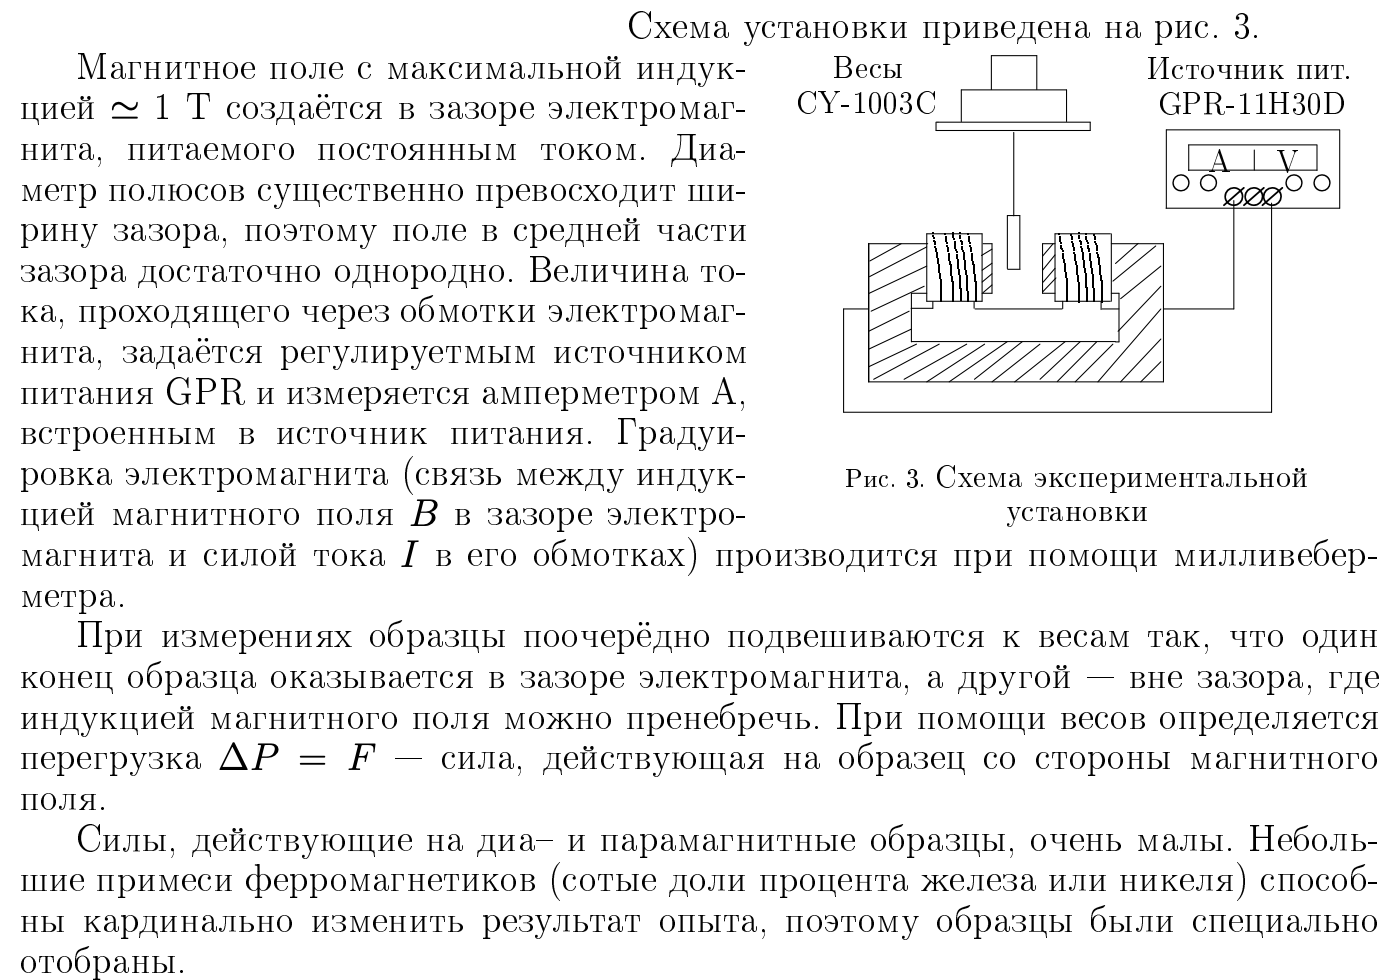
\includegraphics[width = \textwidth]{Picture_1}
	\end{figure}
 	
 	\newpage
 	\section*{{Ход работы}}
 	Данные полученные при калибровке магнита $[B = f(I)]$ \\
 	\[
 	I_{max} = 1,1 A
 	\]
 	\[
 	SN = 72 \, см^2 \, = 72 \cdot 10^{-4} \, м^2
 	\]
 	\[
 	Ф = BSN
 	\]
 	
\begin{table}[!h]
	\centering
	\begin{tabular}{|c|c|c|c|c|c|c|c|}
		\hline
		I, A   & 0,2  & 0,35 & 0,5  & 0,65 & 0,8  & 0,95 & 1,1  \\ \hline
		Ф, мВб & 1,5  & 2,6  & 3,8  & 4,8  & 6    & 6,7  & 7,7  \\ \hline
		B, Тл  & 0,21 & 0,36 & 0,53 & 0,67 & 0,83 & 0,93 & 1,07 \\ \hline
	\end{tabular}
\end{table}

Измерение сил, действующих на образец в магнитном поле. \\
\begin{table}[!h]
	\centering
	\begin{tabular}{|c|c|c|c|c|c|c|c|c|c|c|c|c|c|}
		\hline
		I, A          & 0,2  & 0,35 & 0,5  & 0,65 & 0,8 & 0,95 & 1,1  & 0,95 & 0,8  & 0,65 & 0,5 & 0,35 & 0,2  \\ \hline
		$\Delta$ P, H $\cdot 10^{3}$ & 0,03 & 0,08 & 0,09 & 0,18 & 0,3 & 0,42 & 0,51 & 0,41 & 0,26 & 0,16 & 0,1 & 0,06 & 0,03 \\ \hline
	\end{tabular}
\caption{Измерение сил, действующих на образец из Алюминия}
\end{table}

\begin{table}[!h]
	\centering
	\begin{tabular}{|c|c|c|c|c|c|c|c|c|c|c|c|c|c|}
		\hline
		I, A          & 0,2  & 0,35 & 0,5  & 0,65  & 0,8   & 0,95  & 1,1   & 0,95  & 0,8   & 0,65  & 0,5  & 0,35 & 0,2  \\ \hline
		$\Delta$ P, H $\cdot 10^{3}$ & 0,06 & 0,04 & 0,01 & -0,01 & -0,06 & -0,13 & -0,18 & -0,14 & -0,04 & -0,01 & 0,02 & 0,03 & 0,07 \\ \hline
	\end{tabular}
\caption{Измерение сил, действующих на образец из Меди}
\end{table}

\newpage 
 \section*{Обработка результатов}
 Рассчитаю поле B и построю градуировочную кривую для электромагнита: \\
 \begin{figure}[!h]
 	\centering
 	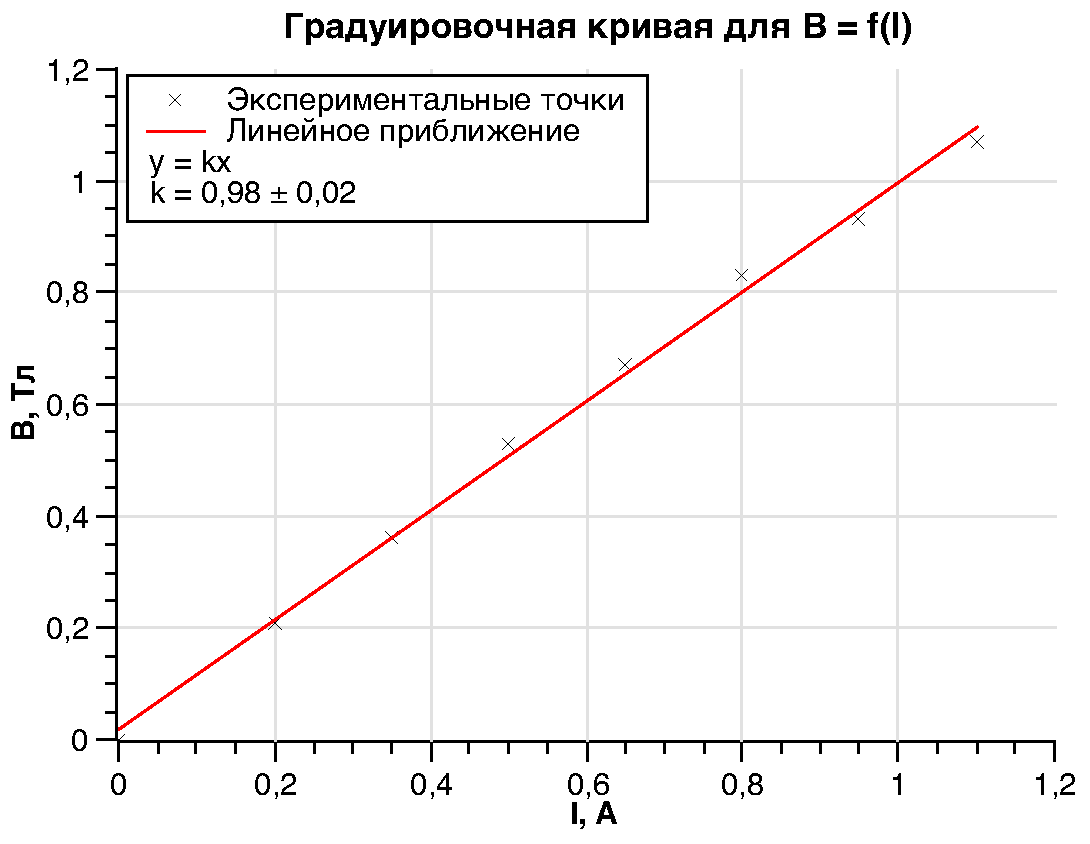
\includegraphics[width=\textwidth]{Graphic_1.pdf} 
 	
 \end{figure}

\noindent Помещая образцы в однородное магнитное поле, по методу Гюи, измеряя
отклонение их равновесной массы без влияния электромагнита, и при разных
токах, то есть при разных значениях магнитной индукции, получаем: \\
\newpage
 \begin{figure}[!h]
	\centering
	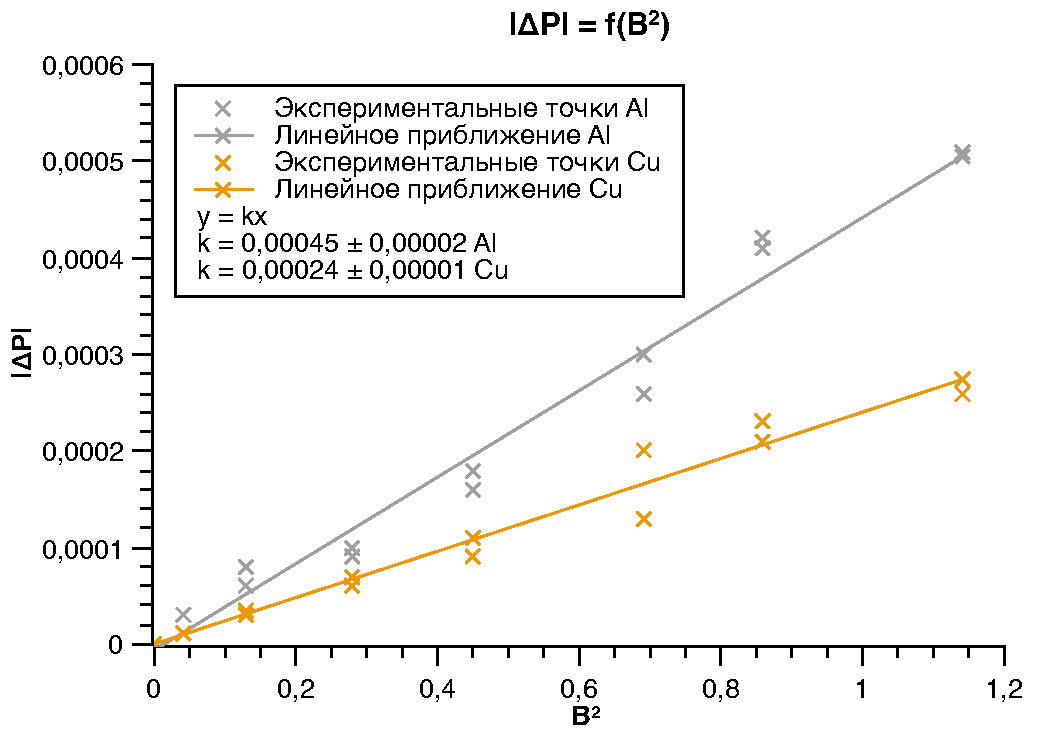
\includegraphics[width=0.9\textwidth]{Graphic_2.pdf} 
	
\end{figure}
\noindent По приближённой формуле и наклонам графиком рассчитаем полученное
значение магнитной восприимчивости.
 \[
 \Delta P = F = \frac{\chi B^2 s}{2 \mu_0}
 \]
\[
\frac{\Delta P}{B^2} = \frac{\chi s}{2 \mu_0}
\]
$\chi_{алюминия} = (19,7 \pm 1,2) \cdot 10^{-6}$ при табличном значении $23 \cdot 10^{-6}$ \\
$\chi_{меди} = (7,7 \pm 0,8) \cdot 10^{-6}$ при табличном значении $10,3 \cdot 10^{-6}$\\
\textbf{Выводы:} Удалось получить значения для магнитной восприимчивости, которые отличаются от табличных в пределах 20 \%. Все вещества подвержены диамагнитному эффекту, который объясняется тем, что при изменении магнитного поля появляется вихревое электрическое, которое сообщает атому ларморовское вращение, из его представления видно, что это одно из проявлений электромагнитной индукции, которое по принципу Ленца препятствует изменениям внешнего приложенного поля В. Поэтому медный образец выталкивается из зазора электромагнита, и его восприимчивость отрицательна. У атомов парамагнетиков орбитальные, спиновые, ядерные моменты не компенсируют друг друга. Однако атомные магнитные моменты расположены беспорядочно, поэтому парамагнитное вещество не обнаруживает магнитных свойств, пока не возникает внешнее поле, которое поворачивает атомы парамагнетика так, что их магнитные моменты устанавливаются преимущественно в направлении поля. Важно отметить, что, как и в случае диамагнетизма, не магнитные силы сообщают подобные изменения, ведь они перпендикулярны к скорости электрона и работы не производят, а взаимодействие между атомами приводит к тому, что столкновения, устанавливающие магнитный момент атомов по полю, (что также поясняется меньшей энергией в таком положении) происходят чаще, чем те, который устанавливают магнитный момент атомов против.
\end{document}